\documentclass[UTF8,fontset=ubuntu]{ctexart}
\usepackage{tikz}
\usetikzlibrary{backgrounds,animations,positioning,fit,shapes.geometric,shapes.misc,shapes.arrows}
\begin{document}

% node
%   A node is typically a rectangle or circle or another simple shape with some text on it
%   参考section 17和section 71

% 语法:
%   \path node <foreach_statement> [<options>] (<name>) at (<coordinate>) {<node_content>}
%     所有node与{之间的选项都是可选的
%     如果node跟在坐标后,则at为非必选,否则at必须指定
%     如果带foreach选项,必须紧跟node关键字,其他可选选项位置不固定

% node坐标系统
% 1.方位
% 显式格式: (node cs:name=<name>,anchor=<anchor>)
%   name - 对已定义node的引用
%   anchor - 引用node指定方位的坐标. 列表如下:
%     north - node内容上侧边框
%     south - node内容下侧边框
%     east - node内容右侧边框
%     west - node内容左侧边框
%     north east - node内容右上角边框
%     north west - node内容左上角边框
%     south east - node内容右下角边框
%     south west - node内容左下角边框
%     center - node内容的中心,默认值
% 隐式格式: (<name>.<anchor>)
\begin{tikzpicture}\begin{tikzpicture}[>=stealth]
    \draw[->] (-2,0) -- (2,0) node[below]{$x$};
    \draw[->] (0,-2) -- (0,2) node[left]{$y$};
    \node [node contents=$p_3$,red,at={(1,1)}];
    \node at (-1,0){$p_2$};
\end{tikzpicture}

    \node[draw] (shape) at (0,2) {class Shape};
    \node[draw] (rect) at (-2,0) {class Rectangle};
    \node[draw] (circle) at (2,0) {class Circle};
    \draw (shape.south) |- (0,1) -| (rect.north);
    \draw (0,1) -| (node cs:name=circle,anchor=north);
%    \draw (0,1) -| (circle.north);
    \fill (0,1) circle [radius=1.2pt];
\end{tikzpicture}

% 2.度
% 显式格式: (node cs:name=<name>,angle=<angle>)
%   angle - 指定角度(非弧度值)
% 隐式格式: (<name>.<angle>)




% 相关参数
% 1.shape - 指定背景形状(section 71). 可选列表: 
%   1)circle - 圆
%   2)rectangle - 矩形. 默认形状
%   下列需要使用shapes.geometric
%   3)diamond - 菱形. 配合参数如下:
%     aspect - 菱形宽度/宽度的比值. 默认为1
%   4)ellipse - 椭圆
%   5)trapezium - 梯形. 配合选项如下:
%     trapezium left angle - 梯形左下角度数. 默认为60
%     trapezium right angle - 梯形右下角度数,默认为60
%     trapezium angle - 梯形左下角和右下角度数
%   6)semicircle - 半圆
%   7)regular polygon - 正多边形. 配合选项如下:
%     regular polygon sides - 正多边形的边数. 默认为5
%   8)star - 多角星. 配合选项如下:
%     star points - 多角星的角数. 默认为5
%     star point height - 圆半径的差距
%     star point ratio - 圆半径之比, 大圆/小圆. 当小圆半径为大圆半径的0.382时,五角星标准
%   9)isosceles triangle - 等腰三角形. 配合选项如下:
%     isosceles triangle apex angle - 顶角度数. 默认30
%   10)kite - 风筝. 配合选项如下:
%     kite upper vertex angel - 顶角度数. 默认120
%     kite lower vertex angle - 底角度数. 默认60
%     kite vertex angle - 顶角和底角度数
%   11)dart - 镖形. 配合选项如下:
%     dart tip angle - 顶部角. 默认45
%     dart tail angle - 底部角. 默认135
%   12)circular sector - 扇形. 配合选项如下:
%     circular sector angle - 圆心角度数
%   13)cylinder - 圆柱体. 配合选项如下:
%     aspect - 圆柱体底部椭圆的半径比(y_radius/x_radius). 默认为1
%     cylinder uses custom fill - 允许填充圆柱体两端和圆柱
%     cylinder end fill - 两端颜色填充
%     cylinder body fill - 圆柱颜色填充
%   下列需要使用shapes.arrows
%   14)single arrow - 单向箭头. 配合选项如下:
%     single arrow tip angle - 箭头夹角角度
%     single arrow head extend - 箭头尾部和线条的距离
%     single arrow head indent - 箭头尾部缩进尺寸
%   15)double arrow - 双向箭头. 配合选项如下:
%     double arrow tip angle - 箭头夹角角度
%     double arrow head extend - 箭头尾部和线条的距离
%     double arrow head indent - 箭头尾部缩进尺寸
%   下列需要使用shapes.misc
%   16)cross out - 交叉删除线
%   17)strike out - 左下角到右上角的单删除线
%   18)rounded rectangle - 宽为圆弧的矩形. 配合选项如下:
%     rounded rectangle arc length - 宽圆弧对应的圆心角度数, 范围为[90,180]
%     rounded rectangle west arc
%     rounded rectangle left arc - 左侧圆弧类型. 可选类型列表:
%       concave - 内凹圆弧
%       convex - 外凸圆弧
%       none - 无圆弧
%     rounded rectangle east arc
%     rounded rectangle right arc - 右侧圆弧类型. 类型参数左侧圆弧
% 2.draw - 背景边框色
% 3.fill - 背景填充色
% 4.rotate - 旋转node
% 5.shape border uses incircle - 边界大小是否由内切圆大小来确定. 值如下:
%   1)true - 由内切圆确定边界大小
%   2)false - 由node content大小确定
% 6.shape border rotate - 只旋转边框. 根据shape border use incircle是否指定,有如下两种情况:
%   1)shape border uses incircle为true,可以旋转边框任意角度
%   2)shape border uses incircle为false,只能旋转边框n * 90度,n为整数
% 7.scale - 扩大/缩小node尺寸
% 8.transform shape - 将外部的图形变化操作引入当前node

\begin{tikzpicture}[scale=3]
    \node at (0,0){example};
    \node[transform shape] at (2,0){exeperiment};
\end{tikzpicture}

% 9.minimum height - 当文字高度(包含inner sep,不包含outer sep)小于指定值时,进行补足;当文字高度(包含inner sep,不包含outer sep)大于等于指定值时,保持原样,不进行裁剪
% 10.minimum width - 类似于minimum height,用于宽度
% 11.minimum size - 同时指定minimum height/width

% 12.behind path - 配合path时,node在path图层下方
%    in front of path - 配合path时,node在path图层上方. 默认选项
%    pgf作图顺序:behind path node -- normal path -- in front of patforh node
% 13.line width - 边框宽度
% 14.double - 边框使用双线
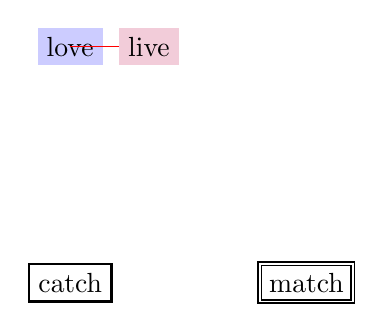
\begin{tikzpicture}[line width=0.6pt]
    \draw[draw=red] (0,0) node[fill=blue!20,behind path]{love} -- (1,0) node[fill=purple!20]{live};
    \node[draw,line width=1pt] at (0,-3){catch};
    \node[draw,double] at (3,-3){match};
\end{tikzpicture}

% 15.inner sep - 文字与背景边框的距离, 默认为1/3em,约3.33pt. 可使用以下参数分别指定x/y轴sep: inner xsep/inner ysep

\begin{tikzpicture}[>=stealth]
    \node[draw] at (1,0){Center};
\end{tikzpicture}this is normal text\\

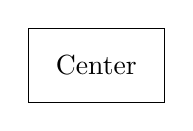
\begin{tikzpicture}[>=stealth]
    \node[inner sep=10pt,draw] at (3,0){Center};
\end{tikzpicture}this is normal text

% 16.outer sep - anchor点从背景边框向外扩散距离, 默认为1/2 * line_width(即边框线中心). 可使用以下参数分别指定x/y轴sep: outer xsep/outer ysep
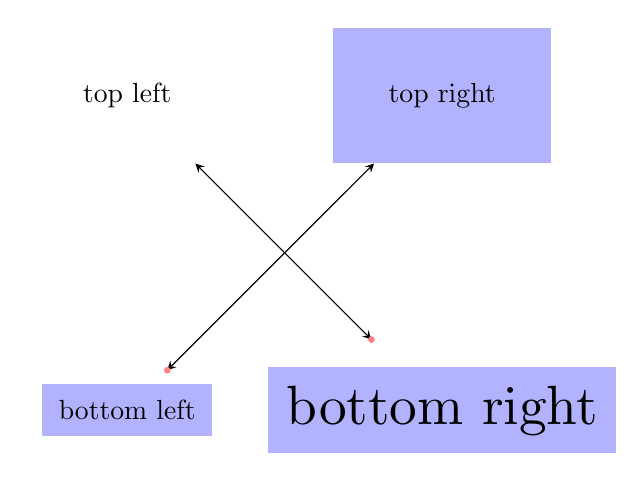
\begin{tikzpicture}[>=stealth]
    \pgfmathsetmacro{\mlength}{2}
    \coordinate (O) at (0,0);
    \node[inner sep=20pt] (A) at (-\mlength,\mlength){top left};
    \node[inner sep=20pt,fill=blue!30] (B) at (\mlength,\mlength){top right};
    \node[inner sep=6pt,line width=10pt,fill=blue!30] (C) at (-\mlength,-\mlength){bottom left};
    \node[scale=2,line width=10pt,fill=blue!30] (D) at (\mlength,-\mlength){bottom right};
    \draw[->] (O) -- (A);
    \draw[->] (O) -- (B);
    \draw[->] (O) -- (C);
    \draw[->] (O) -- (D);
    \fill[red!50] (C.45) circle [radius=1.2pt];
    \fill[red!50] (D.135) circle [radius=1.2pt];
\end{tikzpicture}\\[2cm]
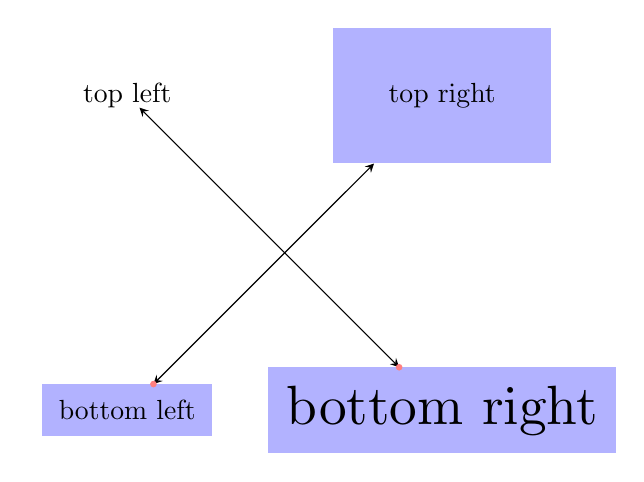
\begin{tikzpicture}[>=stealth]
    \pgfmathsetmacro{\mlength}{2}
    \coordinate (O) at (0,0);
    \node[inner sep=20pt,outer sep=-20pt] (A) at (-\mlength,\mlength){top left};
    \node[inner sep=20pt,fill=blue!30] (B) at (\mlength,\mlength){top right};
    \node[inner sep=6pt,line width=10pt,outer sep=0pt,fill=blue!30] (C) at (-\mlength,-\mlength){bottom left};
    \node[scale=2,line width=10pt,outer sep=0pt,fill=blue!30] (D) at (\mlength,-\mlength){bottom right};
    \draw[->] (O) -- (A);
    \draw[->] (O) -- (B);
    \draw[->] (O) -- (C);
    \draw[->] (O) -- (D);
    \fill[red!50] (C.45) circle [radius=1.2pt];
    \fill[red!50] (D.135) circle [radius=1.2pt];
\end{tikzpicture}

% 17.color - 边框和文字颜色
% 18.text - 指定文本颜色,必须在color后面指定,不然会被color覆盖
% 19.text opacity - 文本透明度
% 20.text width - 文字所占宽度
% 21.text height - 字体所占高度
% 22.text depth - 字体所占深度
% 补充知识:
% node content内容实现多行方式
%   1)使用tabular表格环境
%   2)在使用align参数的前提下,直接使用\\换行
%   3)指定text width参数,达到指定长度后自动换行,此时也可以直接使用\\换行
% 23.align - 多行文本的对齐方式. 可选参数: 
%   1)left - 左对齐
%   2)flush left - 左对齐,尽量避免分词,右侧参差不齐
%   3)right - 右对齐
%   4)flush right - 右对齐,尽量避免分词,左侧参差不齐
%   5)center - 居中对齐
%   6)flush center - 居中对齐,尽量避免分词,两侧参差不齐
%   7)justify - 配合line width使用时,自动调整单词间隔,使两侧对齐
%   8)none - 不进行对齐
% 24.node font - 设置node的字体格式,并且会影响minimum height/minimum width中ex/em单位的大小
%    font - 设置node的字体格式,但不会影响minimum height/minimum width中ex/em单位的大小
\tikz \node [node font=\tiny, minimum height=3em, draw] {tiny};
\tikz \node [node font=\small, minimum height=3em, draw] {small};\\
\tikz \node [font=\tiny, minimum height=3em, draw] {tiny};
\tikz \node [font=\small, minimum height=3em, draw] {small};



% 相关参数
% 25.below - node内容相对于坐标的位置. 可用参数列表如下:
%   1)above - node内容位于坐标上方
%   2)below - node内容位于坐标下方
%   3)left - node内容位于坐标左方
%   4)right - node内容位于坐标右方
%   5)above left - node内容位于坐标左上方
%   6)above right - node内容位于坐标右上方
%   7)below left - node内容位于坐标左下方
%   8)below right - node内容位于坐标右下方
%   9)centered - node内容位于坐标位置
%   备注: [1]below/above/left/right可指定距离值
%         [2]above left/above right/below left/below right也可指定距离值,并且可以使用<dimension_ver> and <dimension_hori>分别指定垂直距离和水平距离,但需要使用positioning库
%         [3]<below>=<dimension> of <coordinate>,可相对于指定坐标的指定方位和长度. 需要使用positioning库
\begin{tikzpicture}[line width=0.6pt]
    \node[above] at (0,0){above};
    \node[below] at (0,0){above};
    \node[below left] at (3,0){this is normal};
    \node[above right=10pt and 2pt] at (3,0){this is normal};
    \fill (0,0) circle [radius=1pt];
    \fill (3,0) circle [radius=1pt];
    \draw (0,-3) -- (3,-3) node[pos=0.33,above]{1/3};
\end{tikzpicture}

% 26.name - 指定node的名称. 与name选项作用一致
\begin{tikzpicture}[>=stealth]
    \draw[->] (-2,0) -- (2,0) node[below]{$x$};
    \draw[->] (0,-2) -- (0,2) node[left]{$y$};
    \node[name=p1] at (1,0){$p_1$};
    \node (p2) at (-1,0){$p_2$};
    \fill (p1.south) circle [radius=2pt];
    \fill (p2) circle [radius=2pt];
\end{tikzpicture}

% 27.alias - 给node赋予一个别称,后续可通过名称或别称访问node

% 28.node contents - 指定node的内容. 之后不再读取其他选项(如: name、node content). 与node content选项作用一致
\begin{tikzpicture}[>=stealth]
    \draw[->] (-2,0) -- (2,0) node[below]{$x$};
    \draw[->] (0,-2) -- (0,2) node[left]{$y$};
    \node at (1,0) [node contents=$p_3$,red];
    \node at (-1,0){$p_2$};
\end{tikzpicture}

% 29.at - 指定node所在坐标. 与at选项作用一致
\begin{tikzpicture}[>=stealth]
    \draw[->] (-2,0) -- (2,0) node[below]{$x$};
    \draw[->] (0,-2) -- (0,2) node[left]{$y$};
    \node [node contents=$p_3$,red,at={(1,1)}];
    \node at (-1,0){$p_2$};
\end{tikzpicture}

% 30.fit - 当前node的尺寸,可以容纳其他node,需要使用fit库
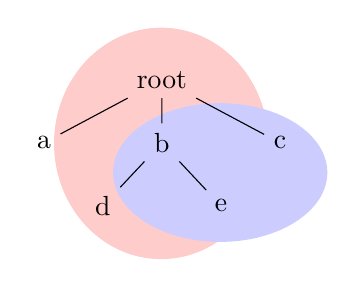
\begin{tikzpicture}[level distance=8mm]
  \node (root) {root}
    child { node (a) {a} }
    child { node (b) {b}
      child { node (d) {d} }
      child { node (e) {e} } }
    child { node (c) {c} };
  \begin{scope}[on background layer]
    \node[fill=red!20,inner sep=0pt,ellipse,fit=(root) (b) (d) (e)] {};
    \node[fill=blue!20,inner sep=0pt,ellipse,fit=(b) (c) (e)] {};
  \end{scope}
\end{tikzpicture}

% 31.pos - node在路径上(前一个坐标到当前坐标)的位置. 如: 0.5代表路径中点. 也可以使用如下参数:
%   1)at start - 类似于pos=0
%   2)very near start - 类似于pos=0.125
%   3)near start - 类似于pos=0.25
%   4)midway - 类似于pos=0.5
%   5)near end - 类似于pos=0.75
%   6)very near end - 类似于0.875
%   7)at end - 类似于pos=1
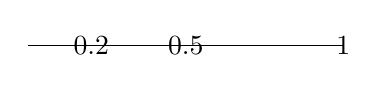
\begin{tikzpicture}
    \draw (-2,0) -- (2,0) node[pos=0.2]{0.2} node[pos=0.5]{0.5} node[pos=1]{1};
\end{tikzpicture}

% 32.auto - node相对于沿路径方向的左侧或右侧. 可选列表:
%   1)left - node位于相对于沿路径方向的左侧
%   2)right - node位于相对于沿路径方向的右侧
\begin{tikzpicture}[>=stealth]
    \draw[->] (-2,0) -- ++(4,0) node[auto=left,pos=0.5]{left} ;
    \draw[->] (-2,-2) -- ++(4,0) node[auto=right,pos=0.5]{right} ;
\end{tikzpicture}

% 33.swap - 切换auto参数的值. 简写方式'
\begin{tikzpicture}[>=stealth,auto=left]
    \draw[->] (-2,0) -- ++(4,0) node[pos=0.5]{left} ;
    \draw[->] (-2,-2) -- ++(4,0) node[swap,pos=0.5]{right} ;
\end{tikzpicture}

% 34.sloped - 旋转node,使node顺着曲线的切线方向. 默认为水平方向
\begin{tikzpicture}[>=stealth]
    \draw[->] (-2,0) .. controls (-2,2) and (2,2) .. (2,0) node[pos=0.3]{0.3} node[sloped,pos=0.6]{0.6};
\end{tikzpicture}




% multi-part node
%   在node内划分多个文字部分, 需要在node content部分使用. 需要特殊shape
%   需要导入shapes.multipart
%   相关shape:
%     1)circle split
%     将circle使用水平线,分为上下两部分. 上部分为text part(main part),下部分为lower part
%     2)circle solidus
%     将circle使用不完整对角线,分为左上/右下两部分. 上部分为text part(main part),下部分为lower part
% update 2025-04-16
%     3)ellipse split
%     将ellipse使用水平线,分为上下两部分. 上部分为text part(main part),下部分为lower part
%     4)rectangle split
%     将rectangle使用水平线或垂直线,分为上下多部分或左右多部分. 分别为text(main part)/two/three/four... part
%     相关参数:
%       rectangle split parts - 指定分为几个part. 默认为4,最多支持分为20份
%       rectangle split horizontal - 是否为水平分割(或垂直分割)
%       rectangle split ignore empty parts - 是否忽略空的部分(不作用于text part)
%       rectangle split empty part width - 设置空part的宽度. 默认为1ex
%       rectangle split empty part height - 设置空part的高度. 默认为1ex
%       rectangle split empty part depth - 设置空part的深度. 默认为0ex
%       rectangle split part align - 使用列表指定每个水平分割(top/bottom/center/base)或垂直分割(left/right/center)part的对齐方式(inner sep对该参数无影响),没有指定的part依照最后一个已指定part的对齐方式. 默认为center
%       rectangle split draw splits - 是否画part之间的分割线. 默认为true
%       rectangle split use custom fill - 是否允许填充part背景. 默认为true
%       rectangle split part fill - 使用列表指定每个part的填充颜色,没有指定的part依照最后一个已指定的颜色. 默认为white
\begin{tikzpicture}[>=stealth,every two node part/.style=red]
    \node[shape=rectangle split,rectangle split horizontal=true,draw] at (1,0){love\nodepart{two}hate\nodepart{three}new\nodepart{four}catch};
\end{tikzpicture}


% update by 2025--4-21





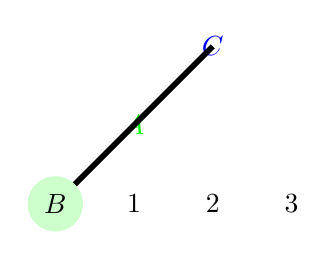
\begin{tikzpicture}
    %   28)label - 在node处额外添加其他node. 格式: [<options>]<angle>:<text>. angle可选列表:
    %     [1]above/below/right/left/above left/above right/below left/below right
    %     [2]center - label node与主node的中心重合
    %     [3]角度值 - label的angle会偏向于45度的整数倍,无法精确定位角度
    %   29)pin - 类似于label,在主node与从node间添加连线
    \path node foreach \x in {1,2,3} at (\x,0) {\x};
    \path node (A) [color=green] at (1,1) {$A$};
    \draw[line width=2pt] (0,0) node[fill=green!20,shape=circle]{$B$} -- (2,2) node[behind path,color=blue]{$C$};
\end{tikzpicture}\\\vspace{1cm}

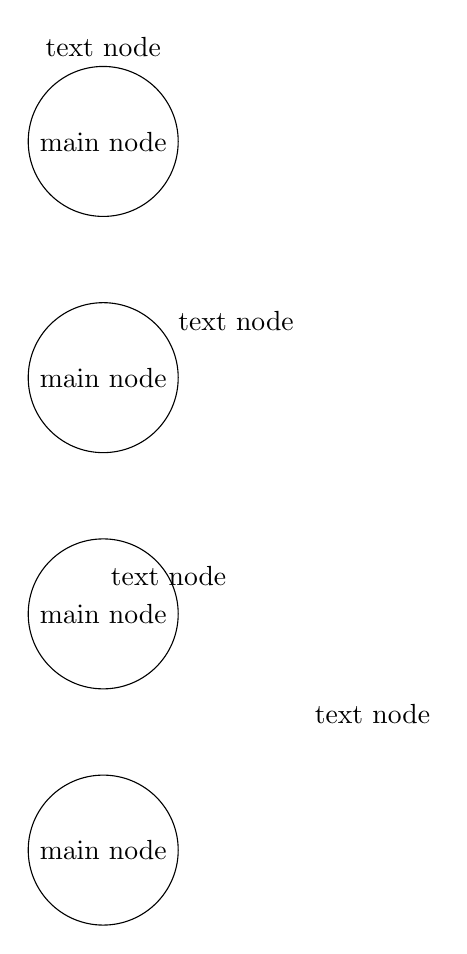
\begin{tikzpicture}
    % 其他node - label
    \path node[circle,draw,label=text node] (A) at (0,0) {main node};
    \path node[circle,draw,label=30:text node] (B) at (0,-3) {main node};
    \path node[circle,draw,label={[centered]30:text node}] (C) at (0,-6) {main node};
    \path node[circle,draw,label={[label distance=2cm]30:text node}] (D) at (0,-9) {main node};
\end{tikzpicture}
\end{document}
